% The 2026 Midterm Elections
% Compile with: latexmk -pdf midterms.tex
\documentclass[aspectratio=169,11pt]{beamer}

\usepackage[T1]{fontenc}
\usepackage{lmodern}
\usepackage{booktabs}
\usepackage{array}
\usepackage{tikz}
\usetikzlibrary{shapes.geometric,positioning,calc,arrows.meta}
\usepackage{pgfplots}
\pgfplotsset{compat=1.18}
\usepackage[most]{tcolorbox}
\graphicspath{{images/}}

% ---------- Colors ----------
\definecolor{navy}{HTML}{1C2541}
\definecolor{oldred}{HTML}{B22234}
\definecolor{oldblue}{HTML}{3C3B6E}
\definecolor{ink}{HTML}{2B2B2B}
\definecolor{muted}{HTML}{8A8F98}
\definecolor{paper}{HTML}{FFFFFF}
\definecolor{dem}{HTML}{2E5FA3}
\definecolor{rep}{HTML}{C0392B}

% ---------- Minimal theme ----------
\setbeamertemplate{navigation symbols}{}
\setbeamercolor{normal text}{fg=ink, bg=paper}
\setbeamercolor{structure}{fg=navy}
\setbeamercolor{frametitle}{fg=navy}
\setbeamercolor{alerted text}{fg=oldred}
\setbeamercolor{footnote}{fg=muted}
\setbeamerfont{frametitle}{size=\Large, series=\bfseries}
\setbeamertemplate{itemize item}{\color{oldred}\textbullet}
\setbeamertemplate{itemize subitem}{\color{muted}--}
\setbeamertemplate{enumerate item}{\color{oldred}\insertenumlabel.}
\setbeamersize{text margin left=1.1cm, text margin right=1.1cm}
\hypersetup{colorlinks=true, urlcolor=dem, linkcolor=navy}

\setbeamertemplate{frametitle}{%
  \vspace*{0.5cm}%
  \usebeamerfont{frametitle}\usebeamercolor[fg]{frametitle}\insertframetitle\par
  \vspace{0.15cm}{\color{navy!15}\rule{\textwidth}{0.4pt}}\par}

\setbeamertemplate{footline}{%
  \hfill{\tiny\color{muted}\insertframenumber}\hspace*{0.6cm}\vspace*{0.35cm}}

% Plain divider at the start of each section
\AtBeginSection{%
  \begin{frame}[plain,noframenumbering]
    \centering
    {\LARGE\bfseries\color{navy}\insertsection}\\[0.6em]
    {\color{oldred}\rule{1.5cm}{0.8pt}}
  \end{frame}}

% "Think" question slides
\newenvironment{thinkframe}{%
  \begin{frame}[plain,noframenumbering,environment=thinkframe]\centering\Large}{\end{frame}}

% ---------- Helpers ----------
% Small grey source line at the bottom of a frame
\newcommand{\source}[1]{%
  \begin{tikzpicture}[remember picture,overlay]
    \node[anchor=south west, font=\tiny, text=muted, text width=0.85\paperwidth, align=left]
      at ($(current page.south west)+(0.6cm,0.25cm)$) {#1};
  \end{tikzpicture}}

% Quote box with a thin red rule on the left
\newtcolorbox{textquote}[1][]{%
  enhanced, frame hidden, boxrule=0pt, sharp corners,
  colback=navy!4, borderline west={2pt}{0pt}{oldred},
  left=10pt, right=8pt, top=6pt, bottom=6pt, fontupper=\itshape, #1}

% Candidate card: photo, name, two lines of bio
\newcommand{\candidate}[3]{%
  \begin{minipage}[t]{\linewidth}\centering
    \includegraphics[height=3.5cm]{#1}\\[0.5em]
    {\large\bfseries\color{navy}#2}\\[0.4em]
    \begin{minipage}{0.9\linewidth}\raggedright\small #3\end{minipage}
  \end{minipage}}

% Big number with a caption
\newcommand{\bignum}[3]{%
  \begin{minipage}[t]{\linewidth}\centering
    {\fontsize{34}{38}\selectfont\bfseries\color{#1}#2}\\[0.3em]
    {\small #3}
  \end{minipage}}

% ---------- Title ----------
\title{The 2026 Midterm Elections}
\author{}
\date{}

\begin{document}

\begin{frame}[plain]
  \begin{columns}[c]
    \begin{column}{0.58\textwidth}
      {\fontsize{30}{34}\selectfont\bfseries\color{navy} Midterm\\Elections}\\[0.8em]
      {\Large\color{muted} The USA, November 2026}\\[0.6em]
      {\color{oldred}\rule{3cm}{1.5pt}}
    \end{column}
    \begin{column}{0.38\textwidth}
      \centering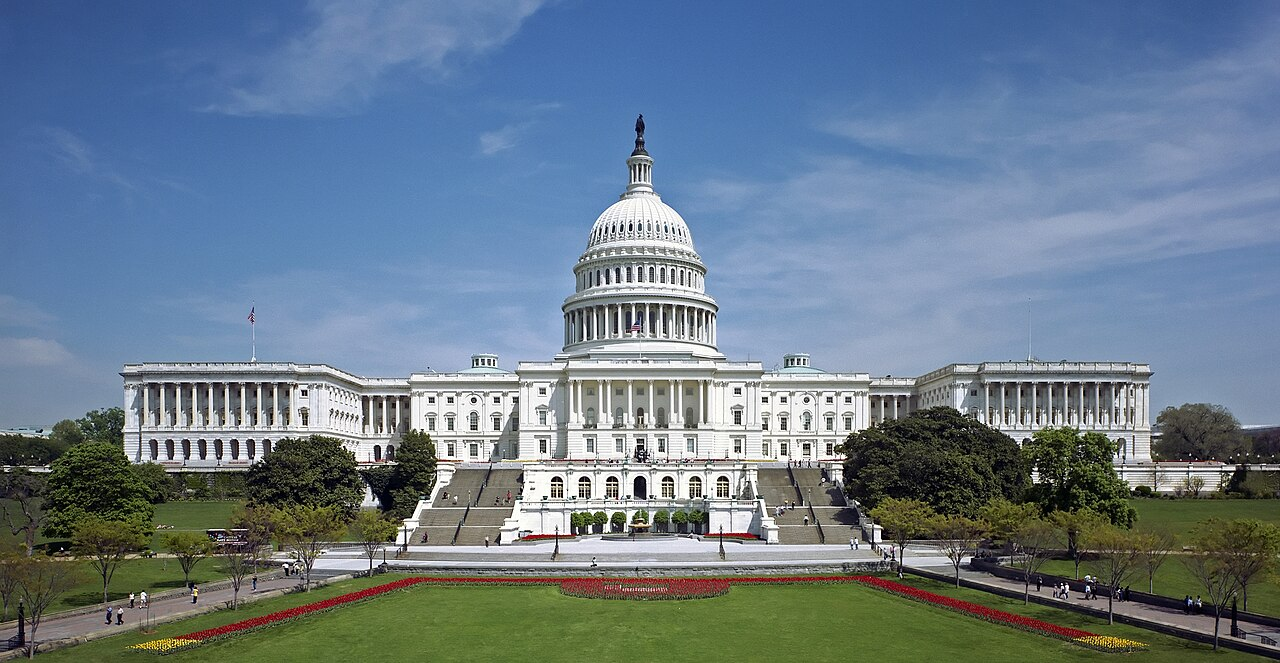
\includegraphics[width=\linewidth]{capitol.jpg}
    \end{column}
  \end{columns}
\end{frame}

% =====================================================================
\section{Warm-up}

\begin{frame}{Who would you vote for?}
  \begin{columns}[T]
    \begin{column}{0.45\textwidth}
      \candidate{jackson.jpg}{Troy Jackson}{%
        \begin{itemize}
          \item Logger from Allagash, northern Maine
          \item Former President of the Maine State Senate
        \end{itemize}}
    \end{column}
    \begin{column}{0.45\textwidth}
      \candidate{collins.jpg}{Susan Collins}{%
        \begin{itemize}
          \item Grew up in Caribou, northern Maine
          \item U.S.\ Senator from Maine since 1997
        \end{itemize}}
    \end{column}
  \end{columns}
\end{frame}

\begin{frame}{What do they stand for?}
  \begin{columns}[T]
    \begin{column}{0.48\textwidth}
      \textbf{\color{dem}Troy Jackson (Democrat)}
      \begin{itemize}\setlength{\itemsep}{0.3em}\small
        \item Medicare for All: government health insurance for everyone
        \item Abolish ICE, the immigration agency he calls ``rogue''
        \item Opposes the war with Iran; would never vote for military aid to Israel
        \item Protect abortion rights in federal law
      \end{itemize}
    \end{column}
    \begin{column}{0.48\textwidth}
      \textbf{\color{rep}Susan Collins (Republican)}
      \begin{itemize}\setlength{\itemsep}{0.3em}\small
        \item Says she votes against her own party more than any other senator
        \item Voted against Trump's ``One Big Beautiful Bill'' (2025)
        \item Supports abortion rights --- but voted to confirm Justice Kavanaugh, who helped overturn \emph{Roe v.\ Wade}
        \item Chairs the committee that controls federal spending
      \end{itemize}
    \end{column}
  \end{columns}
  \vfill
  \begin{center}
    \alert{Do you still feel confident in your vote?}
  \end{center}
\end{frame}

\begin{frame}{Most voters are not well informed}
  \begin{itemize}\setlength{\itemsep}{1.2em}
    \item Only \alert{65\%} of Americans can name all three branches of government
    \item Only about \alert{half} know which party controls each chamber of Congress
    \item Many voters decide based on party, name recognition, or a single ad
  \end{itemize}
  \source{Source: Annenberg Public Policy Center, Civics Surveys (2024, 2026).}
\end{frame}

% =====================================================================
\section{What Is a Midterm?}

\begin{frame}{Basic civics: three branches}
  \relax The U.S.\ government is divided into three \alert{coequal} branches in a system of \alert{checks and balances}.
  \vfill
  \centering
  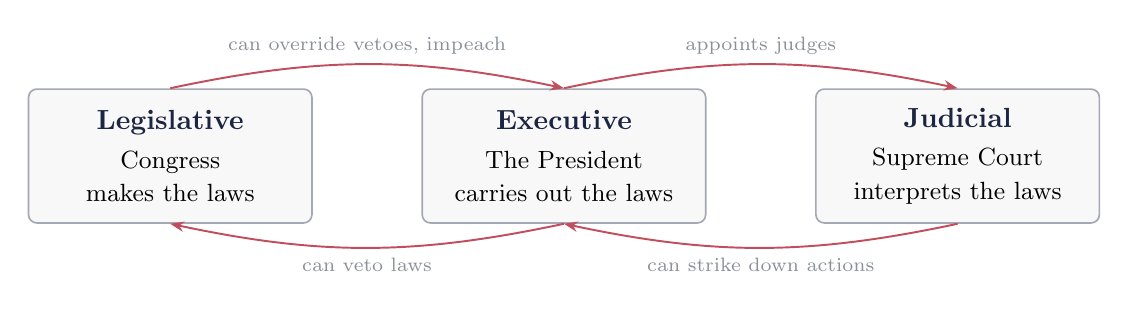
\begin{tikzpicture}[
      box/.style={draw=navy!40, line width=0.6pt, rounded corners=3pt, minimum width=3.6cm,
                  minimum height=1.7cm, align=center, fill=navy!3},
      chk/.style={-{Stealth[length=5pt]}, oldred!80, line width=0.7pt, bend left=12}]
    \node[box] (L) at (0,0) {\textbf{\color{navy}Legislative}\\[0.2em]\small Congress\\\small makes the laws};
    \node[box] (E) at (5,0) {\textbf{\color{navy}Executive}\\[0.2em]\small The President\\\small carries out the laws};
    \node[box] (J) at (10,0) {\textbf{\color{navy}Judicial}\\[0.2em]\small Supreme Court\\\small interprets the laws};
    \draw[chk] (L.north) to node[above, font=\scriptsize, text=muted] {can override vetoes, impeach} (E.north);
    \draw[chk] (E.south) to node[below, font=\scriptsize, text=muted] {can veto laws} (L.south);
    \draw[chk] (E.north) to node[above, font=\scriptsize, text=muted] {appoints judges} (J.north);
    \draw[chk] (J.south) to node[below, font=\scriptsize, text=muted] {can strike down actions} (E.south);
  \end{tikzpicture}
  \vfill
\end{frame}

\begin{frame}{Text Analysis}
  \relax{\small\color{muted} James Wilson, signer of the Constitution and one of the first Supreme Court justices, \emph{Lectures on Law} (1791)\par}
  \vspace{0.3em}
  \begin{textquote}[fontupper=\itshape\small]
    ``The executive as well as the legislative power ought to be restrained. \ldots\ The restraints on the legislative authority, must from its nature, be chiefly internal; that is, they must proceed from some part or division of itself. But the restraints on the executive power are external. These restraints are applied with the greatest certainty, and with greatest efficacy, when the object of restraint is clearly ascertained. This is best done, when one object only, distinguished and responsible, is conspicuously held up to the view and examination of the publick [sic]. \ldots''
  \end{textquote}
\end{frame}

\begin{frame}{Text Analysis}
  \relax{\small\color{muted} James Wilson, \emph{Lectures on Law} (1791), continued\par}
  \vspace{0.3em}
  \begin{textquote}[fontupper=\itshape\small]
    ``\ldots\ In planning, forming and arranging laws, deliberation is always becoming, and always useful. But in the active scenes of government, there are emergencies, in which the man, as, in other cases, the women [sic], who deliberates is lost. Secrecy may be equally necessary as dispatch. But, can either secrecy or dispatch be expected, when, to every enterprise, mutual communication, mutual consultation, and mutual agreement among men, perhaps of discordant views, of discordant tempers, and of discordant interests, are indispensably necessary? How much time will be consumed!''
  \end{textquote}
\end{frame}

\begin{frame}{Compare: the USA and Austria}
  \centering
  \renewcommand{\arraystretch}{1.5}
  \begin{tabular}{@{}>{\raggedright\arraybackslash}p{0.27\textwidth}>{\raggedright\arraybackslash}p{0.32\textwidth}>{\raggedright\arraybackslash}p{0.32\textwidth}@{}}
    \toprule
    & \textbf{\color{oldblue}USA} & \textbf{\color{oldred}Austria} \\
    \midrule
    Who runs the government? & The President & The Chancellor \\
    How are they chosen? & Elected separately from Congress & Needs a majority in parliament (\emph{Nationalrat}) \\
    Head of state & The President (same person) & The Federal President (mostly ceremonial) \\
    National elections & Every 2 years & Every 5 years \\
    \bottomrule
  \end{tabular}
\end{frame}

\begin{frame}{Congress: the legislative branch}
  \begin{columns}[c]
    \begin{column}{0.55\textwidth}
      Congress has \alert{two chambers}:
      \vspace{0.6em}
      \begin{itemize}\setlength{\itemsep}{0.8em}
        \item \textbf{House of Representatives}
          \begin{itemize}
            \item 435 members, 2-year terms
            \item Seats divided by population
          \end{itemize}
        \item \textbf{Senate}
          \begin{itemize}
            \item 100 members, 6-year terms
            \item 2 senators per state, no matter the size
            \item \emph{Filibuster:} most bills need 60 of 100 votes
          \end{itemize}
      \end{itemize}
    \end{column}
    \begin{column}{0.4\textwidth}
      \centering
      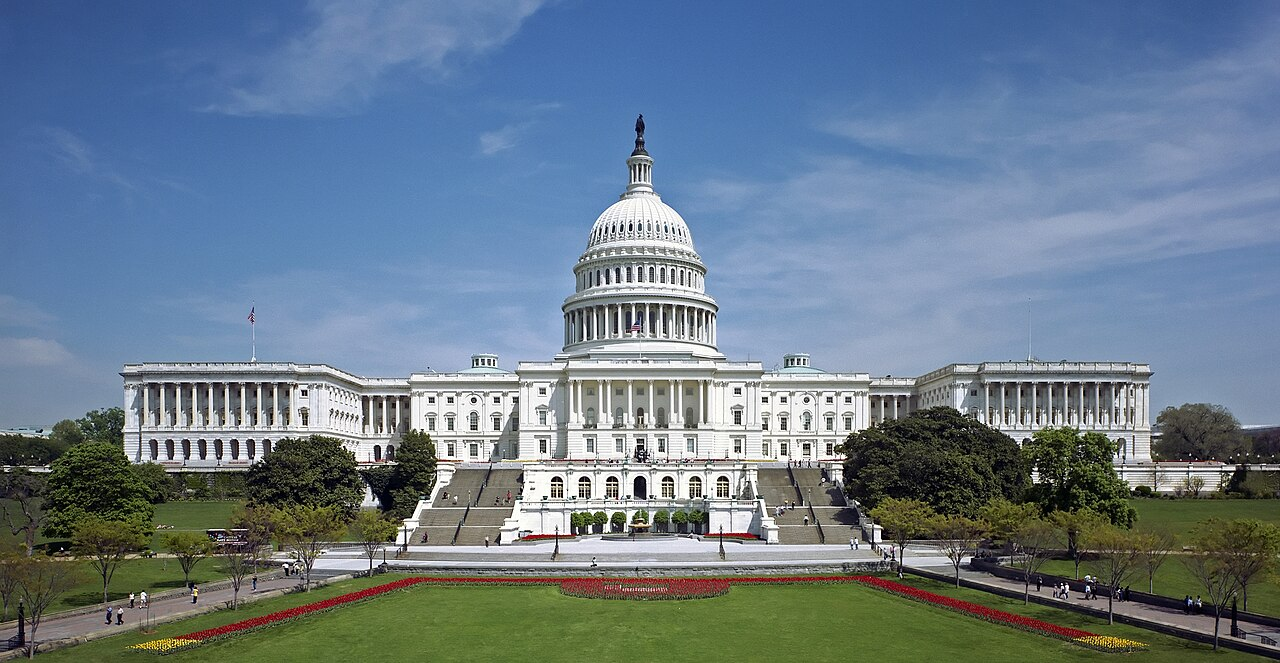
\includegraphics[width=\linewidth]{capitol.jpg}\\[0.2em]
      {\tiny\color{muted} The U.S.\ Capitol, Washington, D.C.\par}
    \end{column}
  \end{columns}
\end{frame}

\begin{frame}{What is a midterm?}
  \begin{itemize}\setlength{\itemsep}{0.7em}
    \item The President serves \textbf{four-year} terms
    \item Midterms are congressional elections \alert{halfway through} a President's term
      \begin{itemize}
        \item All 435 House seats and about a third of the Senate
        \item 2026: Tuesday, \textbf{November 3}
      \end{itemize}
  \end{itemize}
  \vspace{0.6em}
  \textbf{What usually happens?}
  \begin{itemize}\setlength{\itemsep}{0.7em}
    \item Public opinion is ``thermostatic'': it shifts \alert{against the party in power}
    \item In effect, the President's party and positions become more and more unpopular
  \end{itemize}
\end{frame}

\begin{thinkframe}
  {\color{oldred}\textbf{Think}}\\[0.8em]
  Given this trend, what would we expect\\
  to happen in the midterms?
\end{thinkframe}

\begin{frame}{Buyer's remorse}
  \begin{textquote}
    ``He tells you one thing and does just the opposite.''
  \end{textquote}
  {\footnotesize\color{muted}\hfill --- Trump voter in Iowa, on gas and food prices (MS NOW, 2026)}
  \vspace{0.3em}
  \begin{textquote}
    ``It just seems like everything has gone downhill.''
  \end{textquote}
  {\footnotesize\color{muted}\hfill --- Richard, 56, voted Biden in 2020 and Trump in 2024 (NPR focus group, 2026)}
  \vspace{0.3em}
  \begin{textquote}
    ``I've been so disappointed that I'm just going to go straight and just do Democrat, Democrat, Democrat.''
  \end{textquote}
  {\footnotesize\color{muted}\hfill --- Karla, 49, voted Republican in 2024 (NPR focus group, 2026)}
\end{frame}

\begin{frame}{Presidents get less popular}
  \begin{columns}[c]
    \begin{column}{0.62\textwidth}
      \centering
      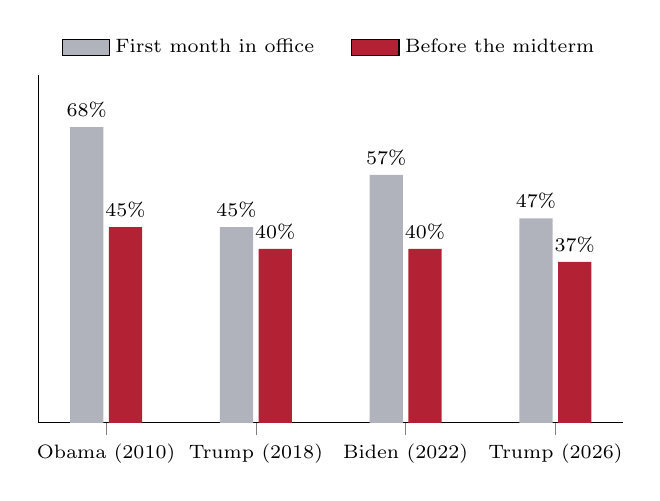
\begin{tikzpicture}
        \begin{axis}[
            ybar, width=9cm, height=6cm, bar width=12pt,
            ymin=0, ymax=80, enlarge x limits=0.15,
            symbolic x coords={Obama (2010),Trump (2018),Biden (2022),Trump (2026)},
            xtick=data, x tick label style={font=\scriptsize},
            axis lines*=left, ytick=\empty,
            nodes near coords={\pgfmathprintnumber\pgfplotspointmeta\%},
            every node near coord/.append style={font=\scriptsize},
            legend style={draw=none, fill=none, font=\scriptsize, at={(0.5,1.02)}, anchor=south, legend columns=2, /tikz/every even column/.append style={column sep=0.4cm}},
            legend cell align=left, area legend]
          \addplot[fill=navy!35, draw=none] coordinates
            {(Obama (2010),68) (Trump (2018),45) (Biden (2022),57) (Trump (2026),47)};
          \addplot[fill=oldred, draw=none] coordinates
            {(Obama (2010),45) (Trump (2018),40) (Biden (2022),40) (Trump (2026),37)};
          \legend{First month in office, Before the midterm}
        \end{axis}
      \end{tikzpicture}
    \end{column}
    \begin{column}{0.34\textwidth}
      \begin{itemize}\setlength{\itemsep}{0.8em}
        \item Every recent President was \alert{less popular} at the midterm than at the start
        \item One in five 2024 Trump voters now say they regret their vote
      \end{itemize}
    \end{column}
  \end{columns}
  \source{Presidential job approval. Sources: Gallup; 2026 value is the polling average as of Oct.\ 16, 2026. Regret figure: Navigator Research (Sept.\ 2026).}
\end{frame}

\begin{frame}{The President's party almost always loses seats}
  \centering
  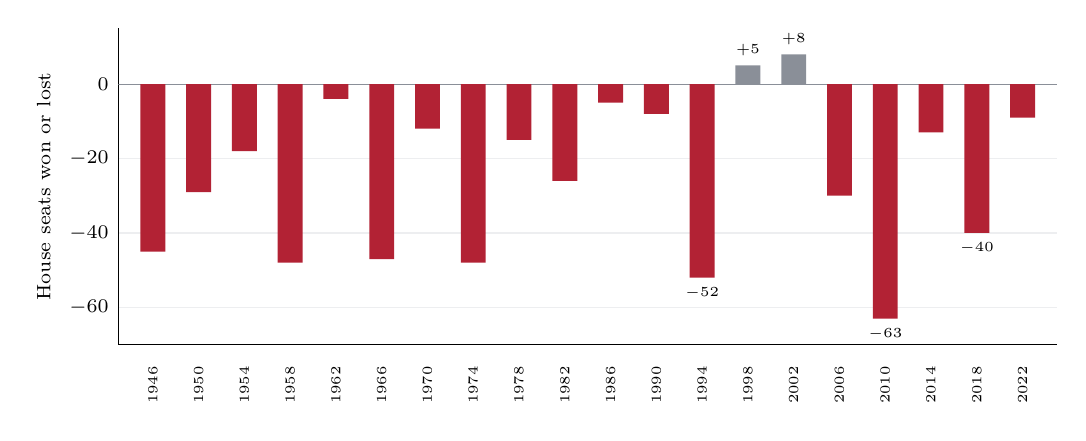
\begin{tikzpicture}
    \begin{axis}[
        ybar, width=13.5cm, height=5.6cm, bar width=9pt,
        ymin=-70, ymax=15, xmin=1943, xmax=2025,
        axis x line*=bottom, axis y line*=left,
        xtick={1946,1950,...,2022}, x tick label style={font=\tiny, rotate=90, anchor=east, /pgf/number format/1000 sep={}},
        ytick={-60,-40,-20,0}, y tick label style={font=\scriptsize},
        ymajorgrids, grid style={navy!8},
        ylabel={\scriptsize House seats won or lost}, tick style={draw=none}]
      \draw[muted] (axis cs:1943,0) -- (axis cs:2025,0);
      \addplot[fill=oldred, draw=none, bar shift=0pt] coordinates {
        (1946,-45) (1950,-29) (1954,-18) (1958,-48) (1962,-4) (1966,-47) (1970,-12)
        (1974,-48) (1978,-15) (1982,-26) (1986,-5) (1990,-8) (1994,-52)
        (2006,-30) (2010,-63) (2014,-13) (2018,-40) (2022,-9)};
      \addplot[fill=muted, draw=none, bar shift=0pt] coordinates {(1998,5) (2002,8)};
      \node[font=\tiny, anchor=north] at (axis cs:1994,-52) {$-$52};
      \node[font=\tiny, anchor=north] at (axis cs:2010,-63) {$-$63};
      \node[font=\tiny, anchor=north] at (axis cs:2018,-40) {$-$40};
      \node[font=\tiny, anchor=south] at (axis cs:1998,5) {+5};
      \node[font=\tiny, anchor=south] at (axis cs:2002,8) {+8};
    \end{axis}
  \end{tikzpicture}

  \vspace{0.3em}
  \small The President's party lost House seats in \alert{18 of 20} midterms since 1946. When the President's approval is below 50\%, the average loss is \alert{37 seats}.
  \source{Sources: University of Michigan Center for Political Studies; Gallup.}
\end{frame}

% =====================================================================
\section{The 2026 Midterms}

\begin{frame}{Where things stand}
  \begin{itemize}\setlength{\itemsep}{0.5em}
    \item Trump is extremely unpopular: about \alert{37\%} approve (one poll: 31\%, his lowest ever)
    \item Democrats are \textbf{heavily favored} to retake the House and \textbf{favored} to take the Senate
  \end{itemize}
  \vspace{1.2em}
  \begin{columns}[T]
    \begin{column}{0.24\textwidth}
      \bignum{dem}{91\%}{House\\\color{muted}Polymarket}
    \end{column}
    \begin{column}{0.24\textwidth}
      \bignum{dem}{94\%}{House\\\color{muted}Nate Silver}
    \end{column}
    \begin{column}{0.24\textwidth}
      \bignum{dem}{64\%}{Senate\\\color{muted}Polymarket}
    \end{column}
    \begin{column}{0.24\textwidth}
      \bignum{dem}{75\%}{Senate\\\color{muted}Nate Silver}
    \end{column}
  \end{columns}
  \vspace{0.6em}
  \begin{center}\footnotesize\color{muted} Chance that Democrats win control, mid-October 2026\end{center}
  \source{Polymarket is a betting market; Nate Silver's Silver Bulletin is a statistical forecast.}
\end{frame}

\begin{frame}{Democrats: a real shot at the Senate}
  \begin{columns}[c]
    \begin{column}{0.45\textwidth}
      \begin{itemize}\setlength{\itemsep}{0.7em}
        \item Republicans hold the Senate \textbf{53--47}
        \item Democrats need to gain \alert{4 seats}
        \item In early 2025, this looked almost impossible
      \end{itemize}
    \end{column}
    \begin{column}{0.52\textwidth}
      \centering
      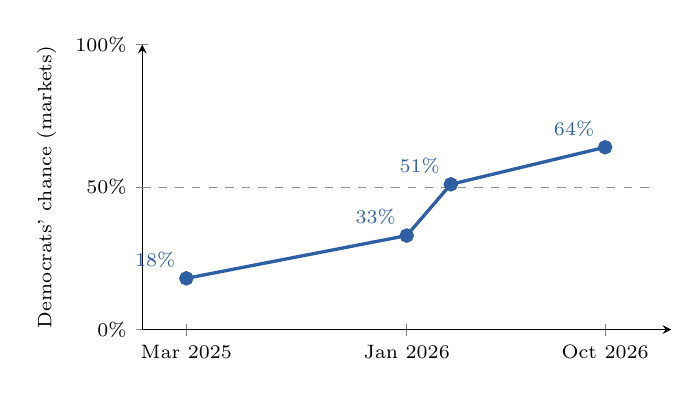
\begin{tikzpicture}
        \begin{axis}[
            width=8.3cm, height=5.2cm,
            xmin=0, xmax=24, ymin=0, ymax=100,
            xtick={2,12,21}, xticklabels={Mar 2025, Jan 2026, Oct 2026},
            x tick label style={font=\scriptsize},
            ytick={0,50,100}, yticklabels={0\%,50\%,100\%}, y tick label style={font=\scriptsize},
            axis lines=left, ylabel={\scriptsize Democrats' chance (markets)},
            nodes near coords={\pgfmathprintnumber\pgfplotspointmeta\%},
            every node near coord/.append style={font=\scriptsize, above left}]
          \draw[muted, dashed] (axis cs:0,50) -- (axis cs:23,50);
          \addplot[very thick, dem, mark=*, mark options={fill=dem}] coordinates
            {(2,18) (12,33) (14,51) (21,64)};
        \end{axis}
      \end{tikzpicture}
    \end{column}
  \end{columns}
  \source{Approximate prediction-market prices (Polymarket and Kalshi), as reported by Yahoo News and Polymarket.}
\end{frame}

\begin{frame}{Democrats: flipping red states?}
  \begin{columns}[T]
    \begin{column}{0.47\textwidth}
      \centering
      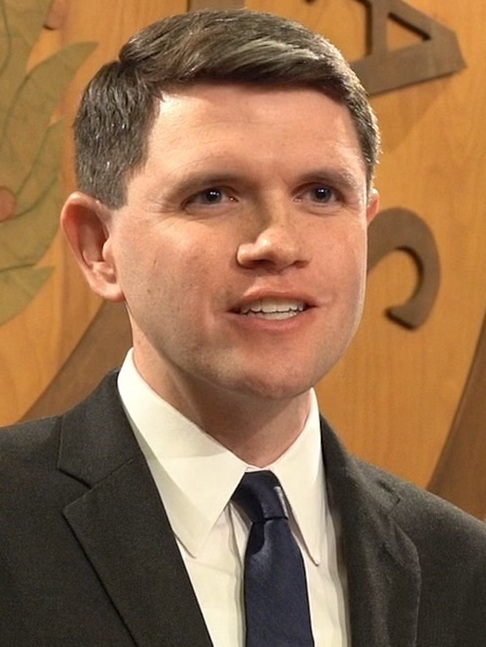
\includegraphics[height=2.4cm]{talarico.jpg}\\[0.4em]
      {\large\bfseries\color{dem}James Talarico}\\[0.1em]
      {\small Texas \textbullet\ vs.\ Ken Paxton (R)}
      \begin{itemize}\small
        \item Texas hasn't elected a Democrat to the Senate since \alert{1988}
        \item Polls: Talarico ahead by about 2 points
      \end{itemize}
    \end{column}
    \begin{column}{0.47\textwidth}
      \centering
      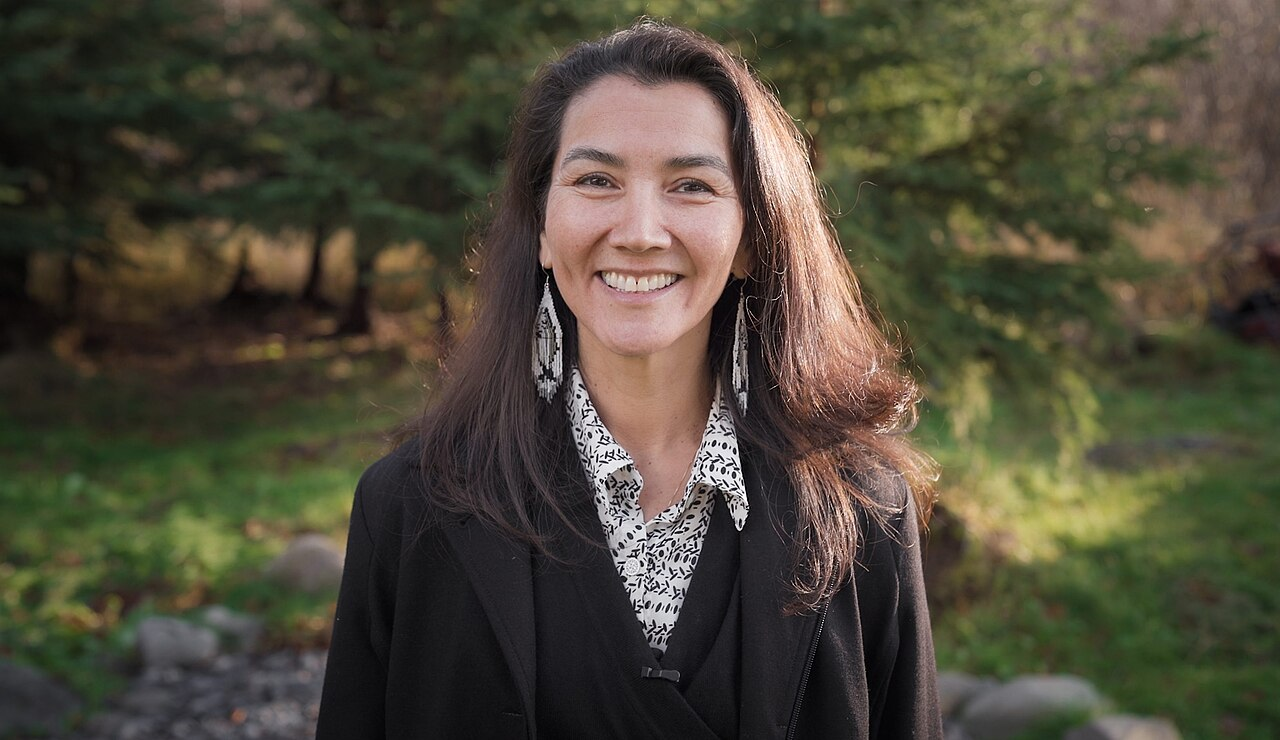
\includegraphics[height=2.4cm]{peltola.jpg}\\[0.4em]
      {\large\bfseries\color{dem}Mary Peltola}\\[0.1em]
      {\small Alaska \textbullet\ vs.\ Sen.\ Dan Sullivan (R)}
      \begin{itemize}\small
        \item Alaska hasn't elected a Democrat to the Senate since \alert{2008}
        \item Polls: very close, Peltola slightly ahead
      \end{itemize}
    \end{column}
  \end{columns}
  \source{Photos: Antonioaesparza, CC BY-SA 4.0; U.S.\ House of Representatives.}
\end{frame}

\begin{frame}{But also: Democratic infighting}
  \begin{columns}[T]
    \begin{column}{0.62\textwidth}
      \textbf{The Maine Senate race}
      \begin{itemize}\setlength{\itemsep}{0.2em}\footnotesize
        \item \textbf{June:} Graham Platner, an oyster farmer and Marine veteran backed by Bernie Sanders, wins the primary over Governor Janet Mills
        \item \textbf{July 10:} Platner drops out after a sexual assault allegation (which he denies) and other scandals: old Reddit posts and a tattoo resembling a Nazi symbol
        \item \textbf{Troy Jackson} had just \alert{lost} the primary for governor (3rd place)
        \item \textbf{July 25:} The party picks Jackson as the new candidate at a convention
        \item Mills refuses to endorse him; Collins has more money in the bank
        \item Today: a \alert{toss-up}, Jackson ahead by about 2 points
      \end{itemize}
    \end{column}
    \begin{column}{0.34\textwidth}
      \centering
      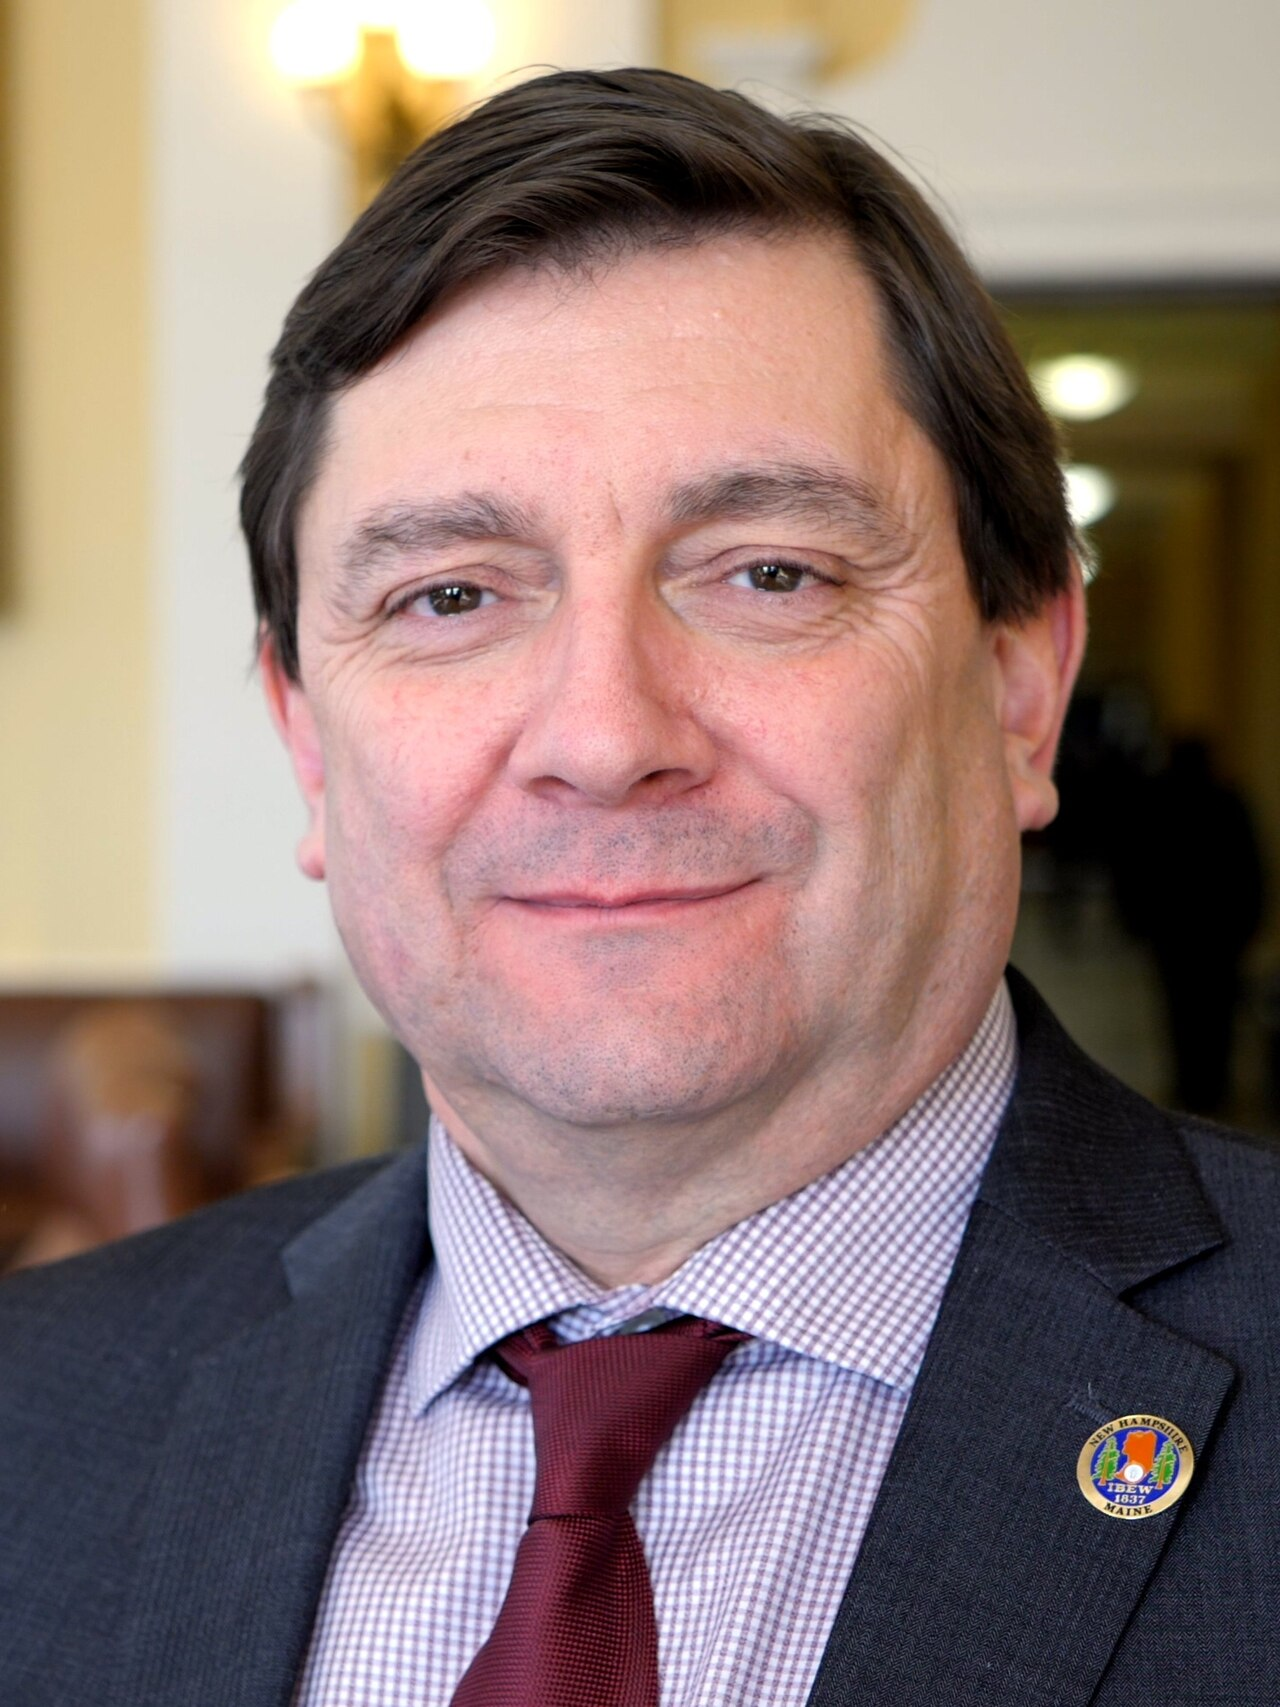
\includegraphics[height=2.5cm]{jackson.jpg}\hspace{0.2cm}%
      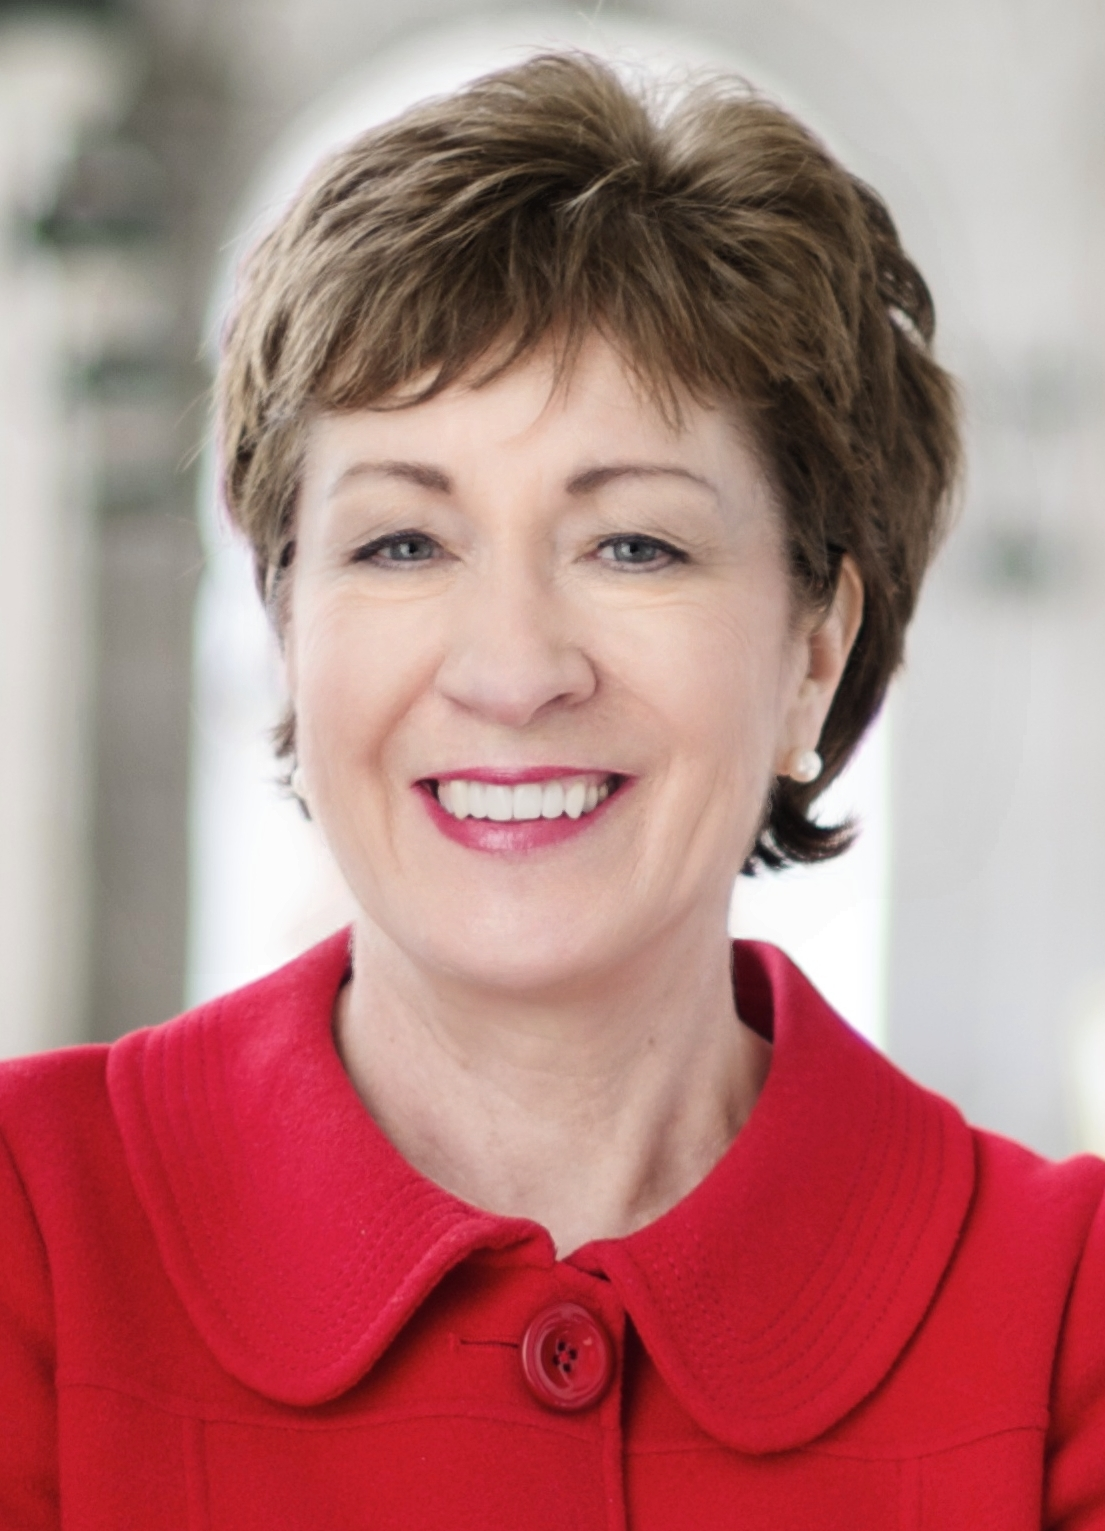
\includegraphics[height=2.5cm]{collins.jpg}\\[0.3em]
      {\scriptsize Jackson (D) \hspace{1.2cm} Collins (R)}
    \end{column}
  \end{columns}
\end{frame}

\begin{frame}{Read aloud}
  \vfill
  \textbf{Candidate A on Candidate B:}
  \begin{textquote}
    \large ``We don't need a celebrity candidate. \ldots\ It didn't work out, so he started the podcast, he wrote the books, and now he's running for Senate.''
  \end{textquote}
  \vspace{1em}
  \textbf{Candidate B's answer:}
  \begin{textquote}
    \large ``Congresswoman, if you enjoy podcasts about public health, I welcome you to take a listen.''
  \end{textquote}
  \vfill
\end{frame}

\begin{frame}{Surprise: they are in the same party!}
  \begin{columns}[c]
    \begin{column}{0.22\textwidth}
      \centering
      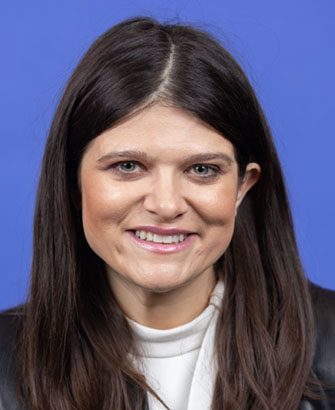
\includegraphics[height=3.2cm]{stevens.jpg}\\[0.3em]
      {\small\bfseries Candidate A:\\ Haley Stevens}
    \end{column}
    \begin{column}{0.36\textwidth}
      \centering
      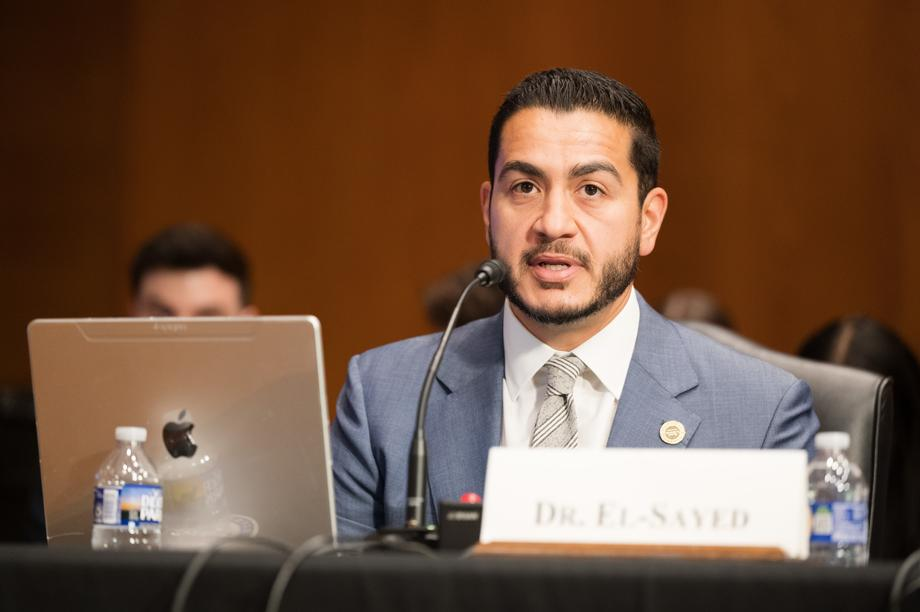
\includegraphics[width=\linewidth]{elsayed.jpg}\\[0.3em]
      {\small\bfseries Candidate B:\\ Abdul El-Sayed}
    \end{column}
    \begin{column}{0.36\textwidth}
      \begin{itemize}\setlength{\itemsep}{0.5em}\small
        \item Both are \alert{Democrats}, from the 2026 Michigan Senate primary
        \item Moderate vs.\ progressive
        \item Stevens and her allies spent about 9 times more on ads
        \item El-Sayed won, 48.5\% to 47.5\%
        \item He now faces Republican Mike Rogers
      \end{itemize}
    \end{column}
  \end{columns}
  \source{Quotes: Michigan Senate primary debate, July 27, 2026. Ad spending: AdImpact via CNBC.}
\end{frame}

\begin{frame}{How have Republicans responded?}
  \begin{itemize}\setlength{\itemsep}{0.9em}
    \item Facing bad polls, Trump and the Republicans have tried to \alert{change the rules} before November
    \item \textbf{Supporters say:} the new rules stop non-citizens from voting and prevent fraud
    \item \textbf{Critics say:} non-citizen voting is extremely rare; the real goal is to make voting harder and \alert{tilt the election}
    \item Three main strategies:
      \begin{enumerate}
        \item New voting laws (the SAVE America Act)
        \item Limiting mail-in voting
        \item Redrawing district maps
      \end{enumerate}
  \end{itemize}
\end{frame}

\begin{frame}{New voting rules}
  \begin{columns}[T]
    \begin{column}{0.48\textwidth}
      \textbf{The SAVE America Act}
      \begin{itemize}\setlength{\itemsep}{0.4em}\small
        \item Would require \textbf{proof of citizenship} (e.g.\ a passport) to register and a \textbf{photo ID} to vote
        \item Passed the House in February, 218--213
        \item Stuck in the Senate: not enough votes to beat the \alert{filibuster}
        \item Trump has demanded that the Senate abolish the filibuster
      \end{itemize}
    \end{column}
    \begin{column}{0.48\textwidth}
      \textbf{Trump's mail-in voting order}
      \begin{itemize}\setlength{\itemsep}{0.4em}\small
        \item Signed March 31, 2026
        \item The Postal Service would \alert{refuse to deliver} mail ballots to anyone not on a government-approved list
        \item September: the Supreme Court blocked it for 2026, 7--2
        \item Mail voting this year works as usual
      \end{itemize}
    \end{column}
  \end{columns}
  \source{Sources: NBC News; Votebeat.}
\end{frame}

\begin{frame}{Mid-decade redistricting}
  \begin{columns}[c]
    \begin{column}{0.55\textwidth}
      \begin{itemize}\setlength{\itemsep}{0.6em}\small
        \item Each state draws its own House districts, normally \textbf{once every 10 years}, after the census
        \item \textbf{Gerrymandering:} drawing district lines so that one party wins more seats than its share of votes
        \item \textbf{2025:} Trump pushed Texas to redraw its map in the middle of the decade to create 5 new Republican seats
        \item California answered with its own Democratic map --- and a ``map war'' began
      \end{itemize}
    \end{column}
    \begin{column}{0.4\textwidth}
      \centering
      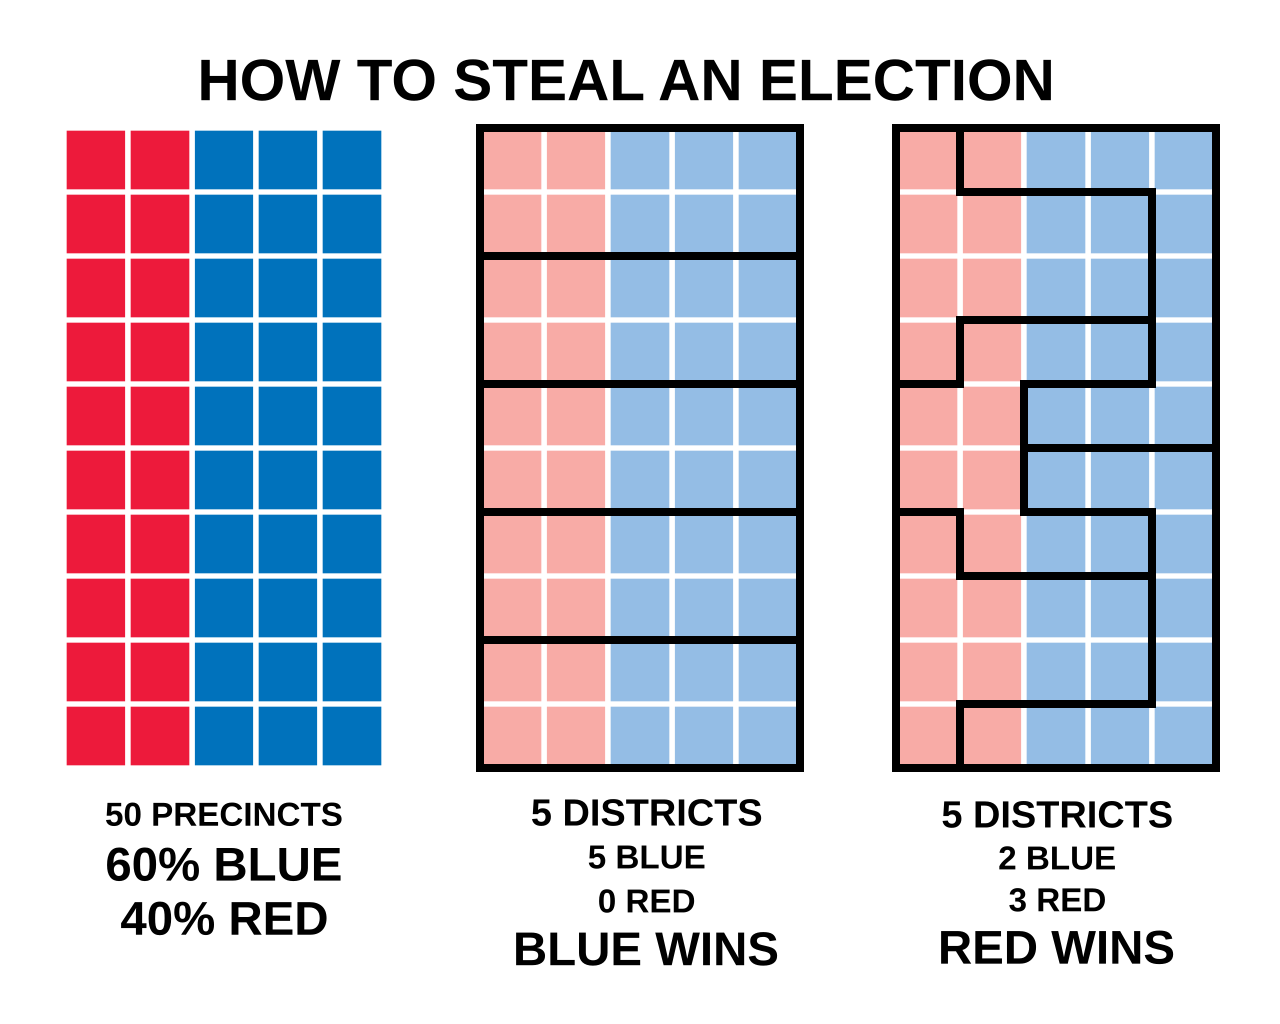
\includegraphics[width=\linewidth]{gerrymander.png}\\[0.1em]
      {\tiny\color{muted} Same voters, different maps. Diagram: Steve Nass, CC BY-SA 4.0\par}
    \end{column}
  \end{columns}
\end{frame}

\begin{frame}{The map war: new seats for 2026}
  \centering
  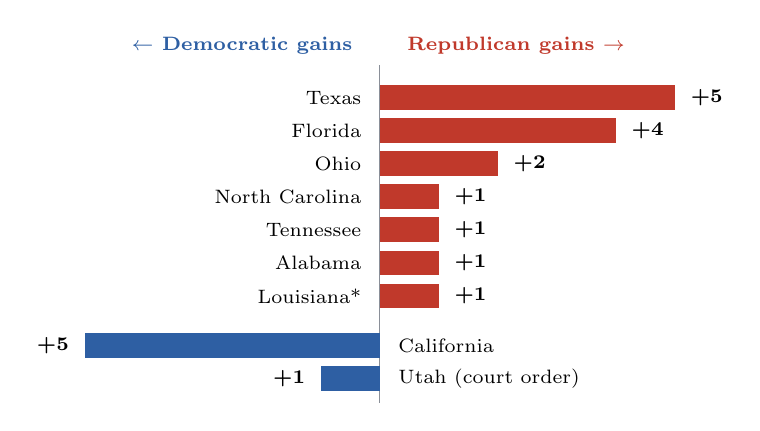
\begin{tikzpicture}[y=-0.42cm, x=0.75cm]
    % axis
    \draw[muted] (0,-0.6) -- (0,9.6);
    \node[font=\scriptsize\bfseries, text=dem, anchor=east] at (-0.3,-1.2) {$\leftarrow$ Democratic gains};
    \node[font=\scriptsize\bfseries, text=rep, anchor=west] at (0.3,-1.2) {Republican gains $\rightarrow$};
    \foreach \i/\st/\v in {0/Texas/5, 1/Florida/4, 2/Ohio/2, 3/North Carolina/1, 4/Tennessee/1, 5/Alabama/1, 6/Louisiana*/1} {
      \fill[rep] (0,\i) rectangle (\v,\i+0.75);
      \node[anchor=east, font=\scriptsize] at (-0.15,\i+0.375) {\st};
      \node[anchor=west, font=\scriptsize\bfseries] at (\v+0.1,\i+0.375) {+\v};
    }
    \foreach \i/\st/\v in {7.5/California/5, 8.5/Utah (court order)/1} {
      \fill[dem] (0,\i) rectangle (-\v,\i+0.75);
      \node[anchor=west, font=\scriptsize] at (0.15,\i+0.375) {\st};
      \node[anchor=east, font=\scriptsize\bfseries] at (-\v-0.1,\i+0.375) {+\v};
    }
  \end{tikzpicture}

  \vspace{0.4em}
  \small Net effect: roughly \alert{+9 seats for Republicans}. Virginia's Democratic map was struck down by its state court; Indiana Republicans refused to redraw.
  \source{Estimated seat gains. *Louisiana's map is being challenged in court. Source: Wikipedia, ``2025--2026 United States redistricting.''}
\end{frame}

\begin{frame}{Money: Republicans have far more cash}
  \centering
  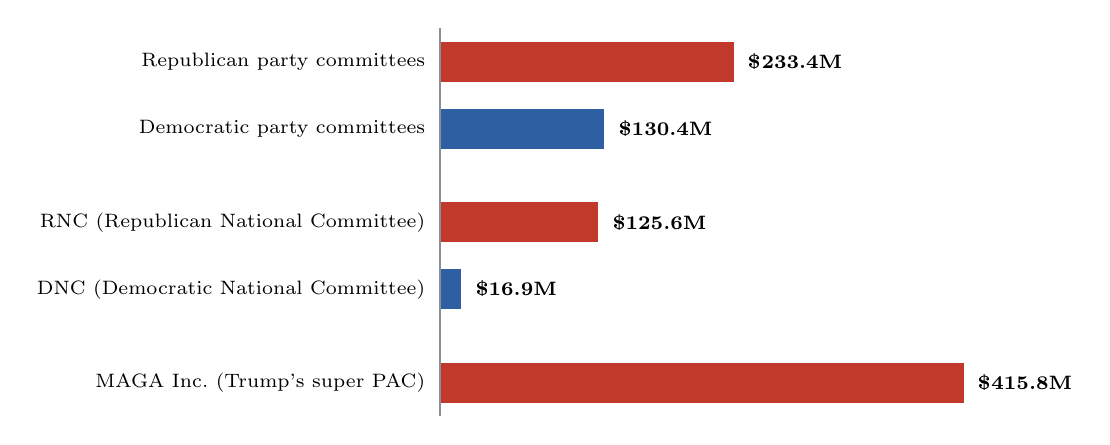
\begin{tikzpicture}[x=0.016cm, y=-0.85cm]
    \foreach \i/\lab/\v/\col in {
        0/{Republican party committees}/233.4/rep,
        1/{Democratic party committees}/130.4/dem,
        2.4/{RNC (Republican National Committee)}/125.6/rep,
        3.4/{DNC (Democratic National Committee)}/16.9/dem,
        4.8/{MAGA Inc.\ (Trump's super PAC)}/415.8/rep} {
      \fill[\col] (0,\i) rectangle (\v,\i+0.6);
      \node[anchor=east, font=\scriptsize] at (-4,\i+0.3) {\lab};
      \node[anchor=west, font=\scriptsize\bfseries] at (\v+4,\i+0.3) {\$\v M};
    }
    \draw[muted] (0,-0.2) -- (0,5.6);
  \end{tikzpicture}

  \vspace{0.5em}
  \small The DNC is also \alert{\$17.6 million in debt}.
  \source{Cash on hand at the end of August 2026. Source: FEC filings via CNBC.}
\end{frame}

\begin{frame}{Money: where does it come from, where does it go?}
  \begin{columns}[T]
    \begin{column}{0.48\textwidth}
      \textbf{Where it comes from}
      \begin{itemize}\setlength{\itemsep}{0.4em}\small
        \item \textbf{Billionaires:} Elon Musk is the biggest donor of 2026; Miriam Adelson gave about \$68 million
        \item \textbf{Tech \& crypto:} the founders of Andreessen Horowitz gave \$115 million; the crypto super PAC Fairshake has over \$140 million
        \item \textbf{But:} many Democratic \emph{candidates} raise more from small online donors (Jackson: \$20 million+)
      \end{itemize}
    \end{column}
    \begin{column}{0.48\textwidth}
      \textbf{Where it goes}
      \begin{itemize}\setlength{\itemsep}{0.4em}\small
        \item Super PACs can spend \alert{unlimited} money, as long as they don't coordinate with candidates
        \item Musk gave \alert{\$158 million} to the Senate Leadership Fund, which sent \$158 million to Texas to fight Talarico
        \item Most of it pays for TV and online ads in battleground states
      \end{itemize}
    \end{column}
  \end{columns}
  \source{Sources: Washington Post; Forbes; Public Citizen; AP; FEC.}
\end{frame}

\begin{frame}{If we have time: the ads}
  \relax See how the money plays out in the Senate battlegrounds:
  \vspace{1em}
  \begin{itemize}\setlength{\itemsep}{0.9em}
    \item \textbf{Maine:} \href{https://www.youtube.com/results?search_query=Troy+Jackson+Susan+Collins+Senate+ad}{Troy Jackson vs.\ Susan Collins}
    \item \textbf{Texas:} \href{https://www.youtube.com/results?search_query=Talarico+Paxton+Senate+ad}{James Talarico vs.\ Ken Paxton}
    \item \textbf{Alaska:} \href{https://www.youtube.com/results?search_query=Peltola+Sullivan+Senate+ad}{Mary Peltola vs.\ Dan Sullivan}
    \item \textbf{Michigan:} \href{https://www.youtube.com/results?search_query=El-Sayed+Mike+Rogers+Senate+ad}{Abdul El-Sayed vs.\ Mike Rogers}
  \end{itemize}
\end{frame}

% =====================================================================
\section{Final Activity}

\begin{frame}{Now you are informed voters}
  \begin{columns}[c]
    \begin{column}{0.3\textwidth}
      \centering
      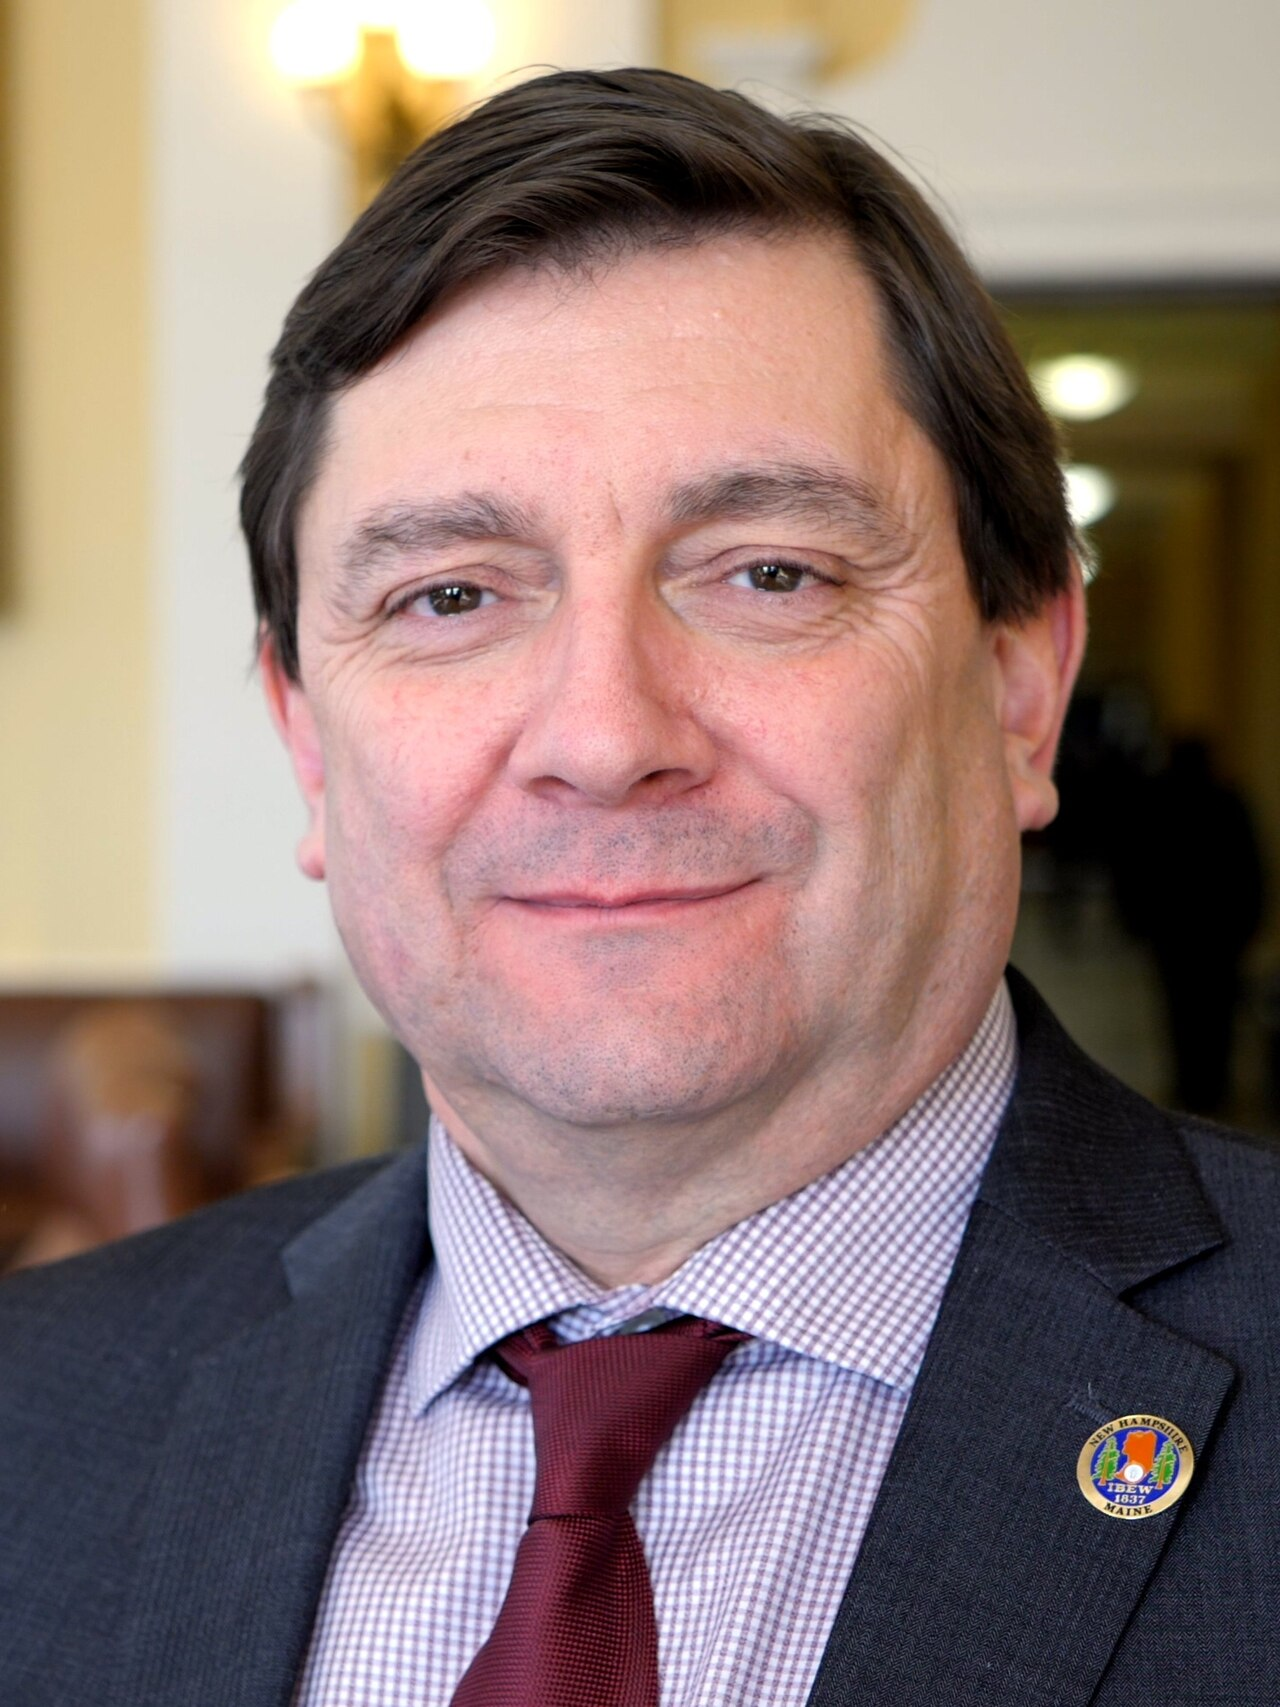
\includegraphics[height=3.6cm]{jackson.jpg}\\[0.3em]
      {\bfseries\color{dem}Troy Jackson (D)}
    \end{column}
    \begin{column}{0.3\textwidth}
      \centering
      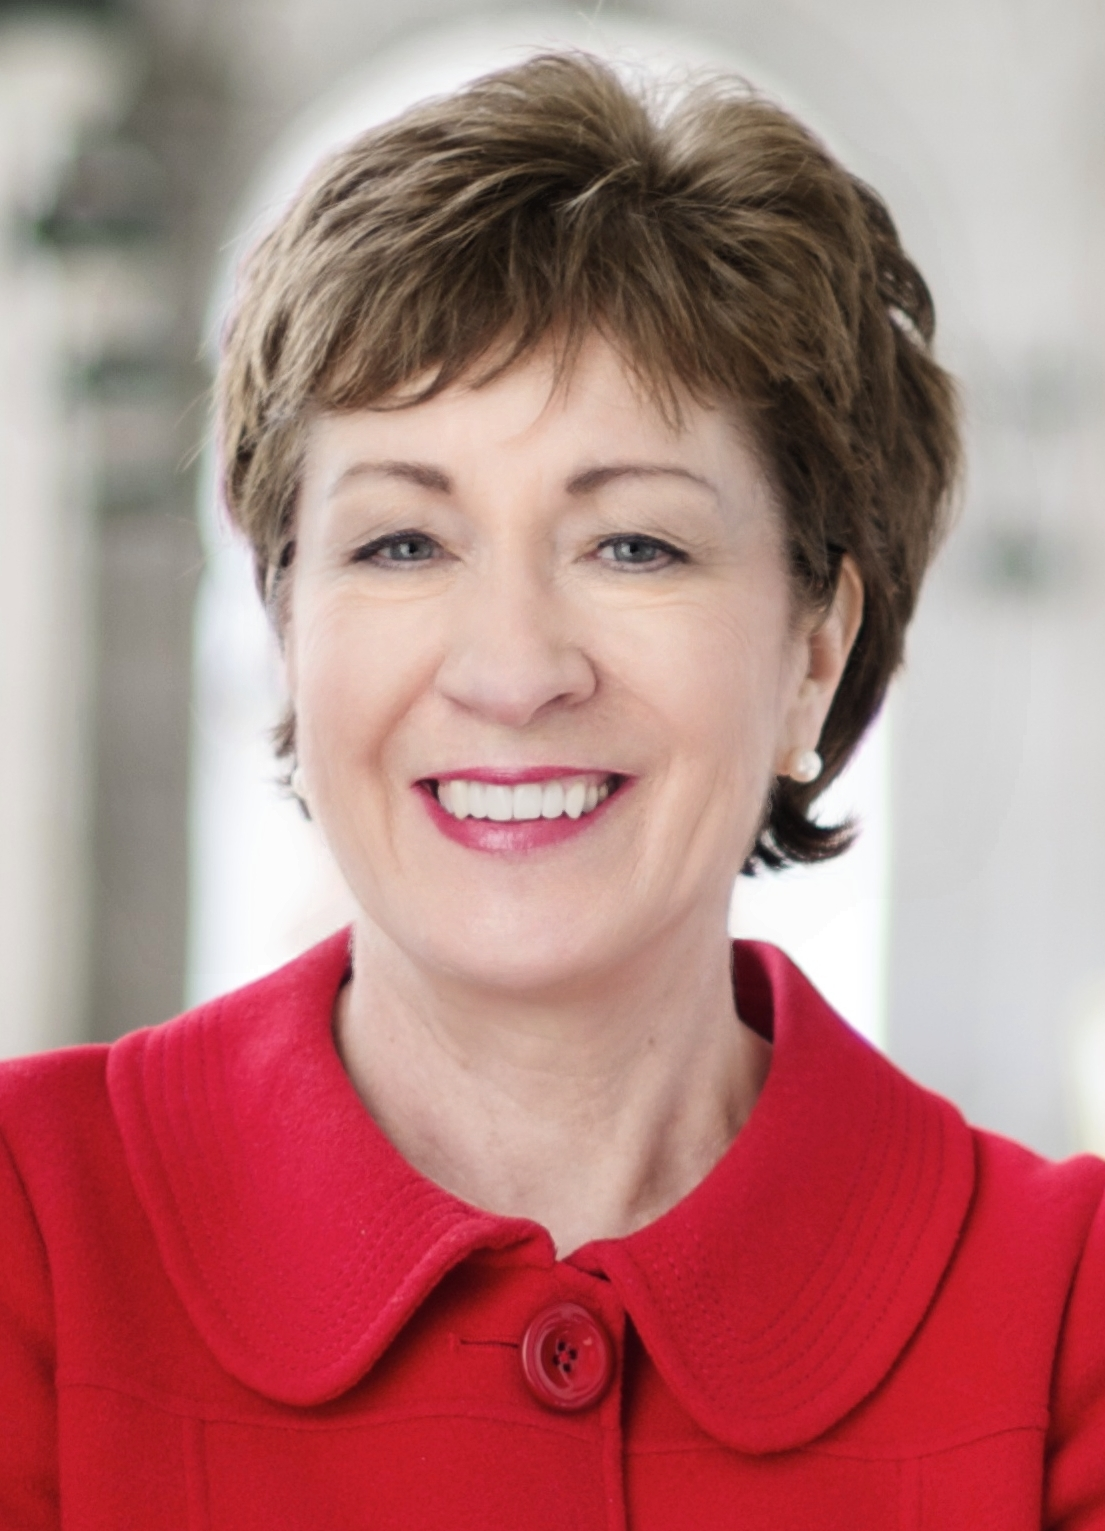
\includegraphics[height=3.6cm]{collins.jpg}\\[0.3em]
      {\bfseries\color{rep}Susan Collins (R)}
    \end{column}
    \begin{column}{0.34\textwidth}
      \begin{itemize}\setlength{\itemsep}{0.8em}
        \item Revisit your choice from the start of the lesson
        \item Choose a candidate
        \item \alert{Justify your answer!}
      \end{itemize}
    \end{column}
  \end{columns}
\end{frame}

\end{document}
